\documentclass{article}
\usepackage{graphicx} % Required for inserting images
\usepackage[a4paper, left=3cm, right=2cm, top=2cm, bottom=2cm]{geometry}
\usepackage{float}
\usepackage{subcaption}  % For subfigure support
\usepackage{subfigure}


\title{Lab2 Report}
\author{Nguyen Thanh Tung - 2440047}
\begin{document}
\maketitle

We implement the read data function to open a csv file read each line and split the input and output data into two list.


\begin{figure}[H]
    \centering
    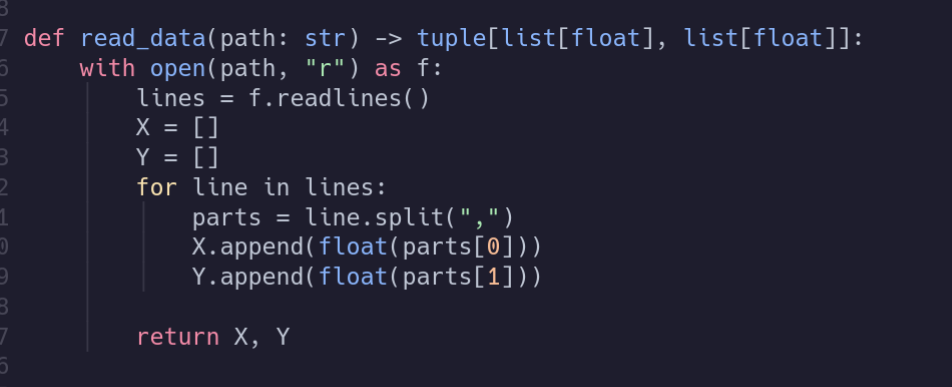
\includegraphics[width=0.5\linewidth]{read_data.png}
    \caption{Read data}
    \label{fig:enter-label}
\end{figure}

The predict function will take a batch of input data and compute for each data \(y=wx+b\). The loss function is used to calculate the mean square error of the model prediction. The dlw function calculate the derivative of the loss function with respect to the weight w. The dlb calculate the derivative of the loss function with respect to the bias b. 

\begin{figure}[H]
    \centering
    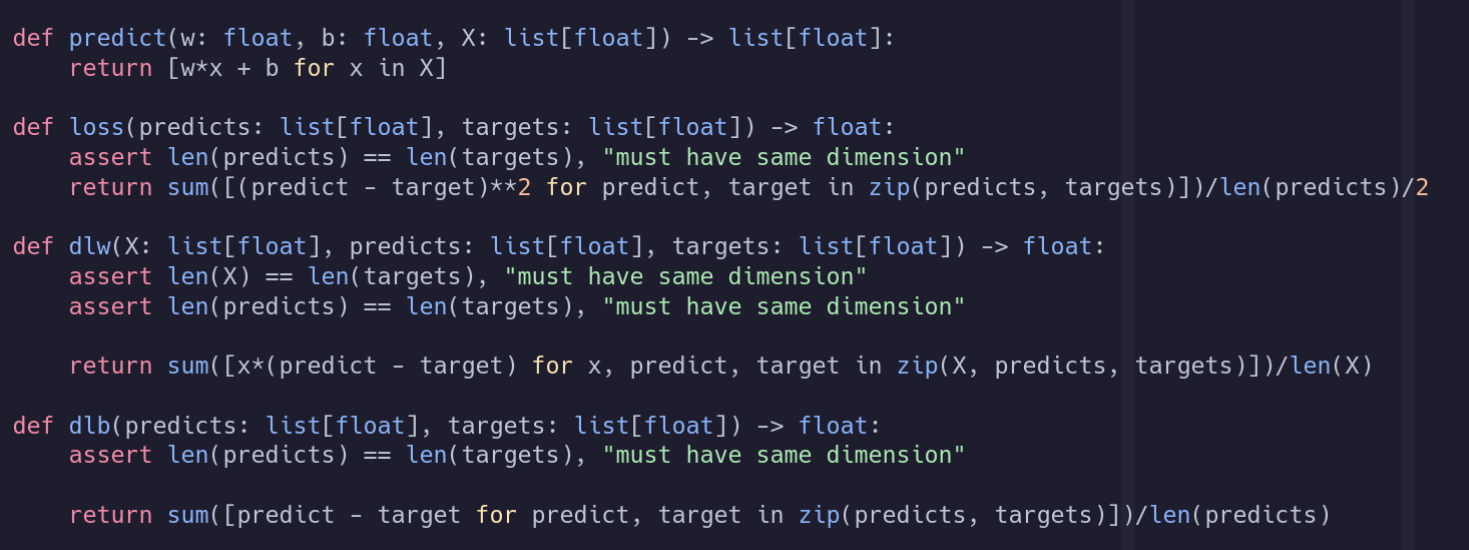
\includegraphics[width=0.5\linewidth]{impl.png}
    \caption{Model implementation}
    \label{fig:enter-label}
\end{figure}

To train the model, in this cased we used batch gradient descent. For each epoch, we calculate the loss of the model prediction on the whole dataset and compute the derivative of the loss and update the weight and bias accordingly. The weight and bias is initialize to a small number near zero.

\begin{figure}[H]
    \centering
    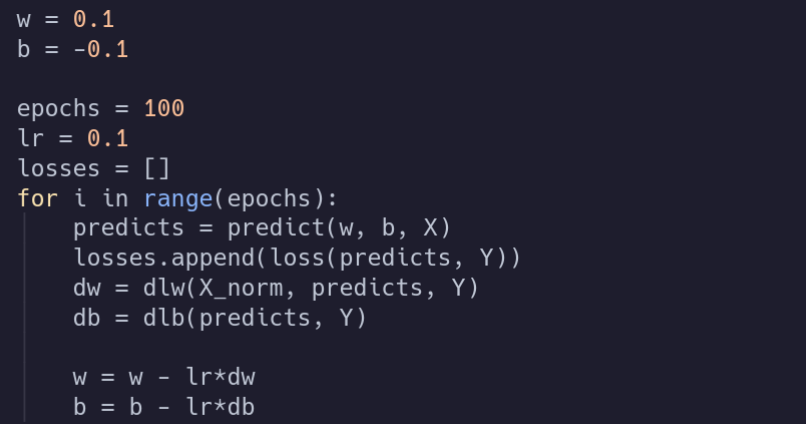
\includegraphics[width=0.5\linewidth]{train.png}
    \caption{Training code}
    \label{fig:enter-label}
\end{figure}

We try to analyze the impact of learning rate on the training of the model. 
With a learning rate of 0.1 we see that the model can not learn and even diverge, the loss function grows exponentially. This is due to the data having a large range [10, 80], [55, 150] so the loss and gradient also has a large range. There for the learning rate of 0.1 will update the parameter too much leading to the divergence of the loss function.

\begin{figure}[H]
    \begin{subfigure}{0.5\linewidth}
        \centering
        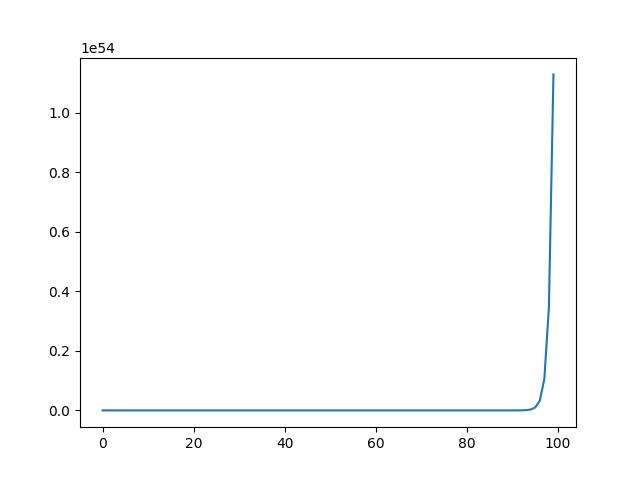
\includegraphics[width=\linewidth]{loss_train_no_norm_0.1lr.jpg}
        \caption{Loss function}
    \end{subfigure}
    \begin{subfigure}{0.5\linewidth}
        \centering
        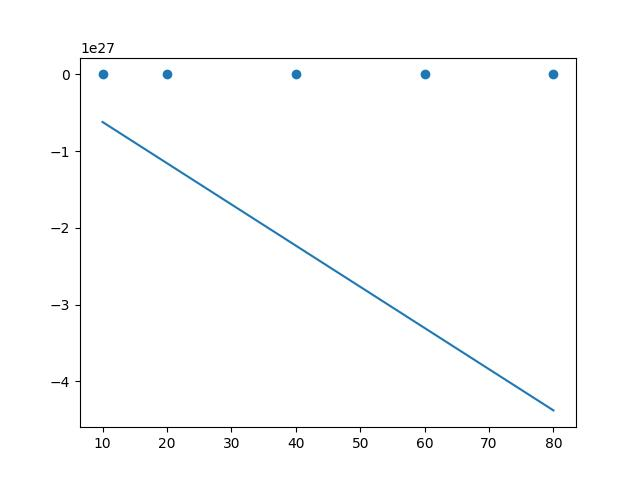
\includegraphics[width=\linewidth]{output_train_no_norm_0.1lr.jpg}
        \caption{Model prediction}
    \end{subfigure}
    \caption{Training results with learning rate of 0.1}
    \label{fig:enter-label}
\end{figure}

We have to choose a significantly smaller learning rate to allow the model to learn. With a learning rate of 0.0005 the model can predict well the linear trend of the date. However, the model only converged after about 4000 epochs.
We also tried a higher learning rate to accelerate the training process but any higher learning rate will cause the loss function to diverge or oscillate.

\begin{figure}[H]
    \begin{subfigure}{0.5\linewidth}
    \centering
        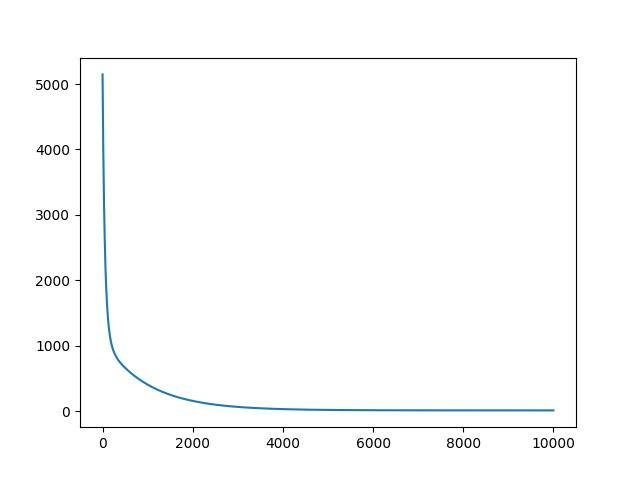
\includegraphics[width=\linewidth]{loss_train_no_norm_0.0005lr.jpg}
        \caption{Loss function}
    \end{subfigure}
    \begin{subfigure}{0.5\linewidth}
    \centering
        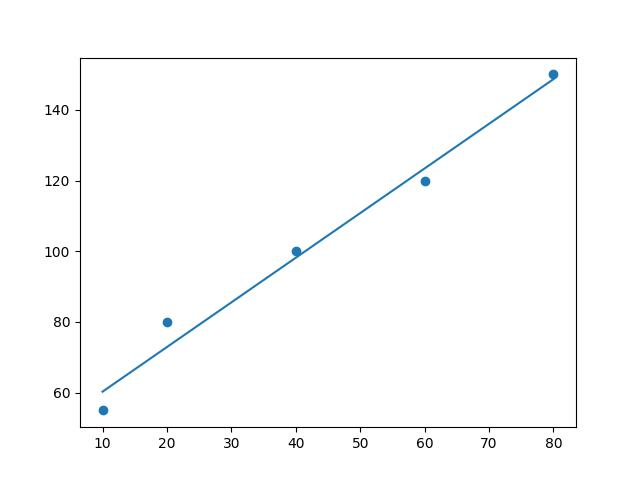
\includegraphics[width=\linewidth]{output_train_no_norm_0.0005lr.jpg}
        \caption{Model prediction}
    \end{subfigure}
    \caption{Training results with learning rate of 0.0005}
    \label{fig:enter-label}
\end{figure}

To help the model to learn better, we have to address the large range of the input and output data. We implemented normalization. The mean and standard deviation of the input and output data is calculated. The data is then shifted and scaled with the formulas:
\[\mu_x = \frac{\sum x}{N}\]
\[\mu_y = \frac{\sum y}{N}\]
\[\sigma_x = \sqrt{\frac{\sum (x - \sigma_x)^2}{N + 1}}\]
\[\sigma_y = \sqrt{\frac{\sum (y - \sigma_y)^2}{N + 1}}\]
\[x_{norm} = \frac{x - \mu_x}{\sigma_x}\]
\[y_{norm} = \frac{y - \mu_y}{\sigma_y}\]
The standard deviation calculation use the normalization factor of \(N + 1\) (with \(N\) is the number of data point) because we are calculating the sample standard deviation and not the real population standard deviation so add 1 to the normalization factor will better model the real value.

After the transformation, the normalize data will follow normal distribution \(N(0, 1)\) with the mean of 0 and standard deviation of 1.

This normalization step will help the loss function to not grow to big and we can more easily choose a learning rate. Consequently the model will have better learning result.

\begin{figure}[H]
    \centering
    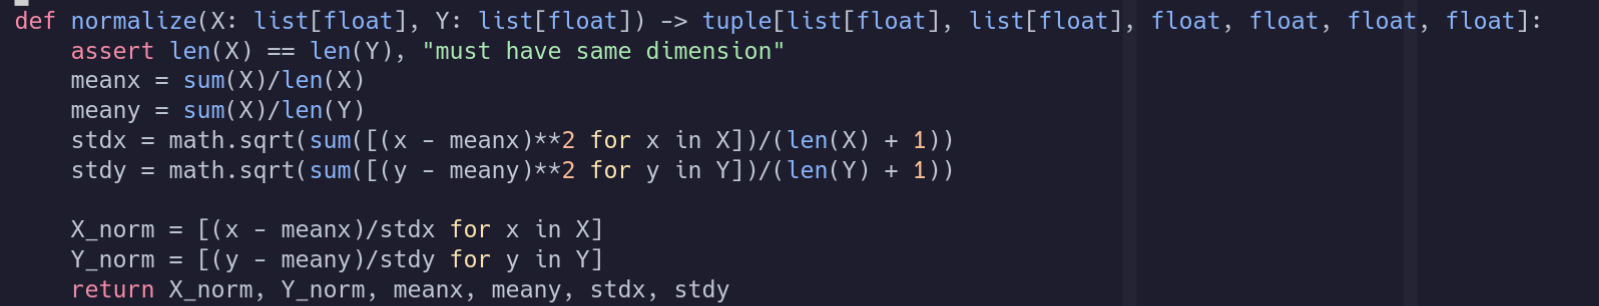
\includegraphics[width=0.75\linewidth]{normallize.png}
    \caption{Normalization code}
    \label{fig:enter-label}
\end{figure}

We will use the normalized input and output data to train the model. After the training complete, if we want to predict new data, we can use the calculated to mean and standard deviation values of the input and output data to scale this new data and the predicted output.

\begin{figure}[H]
    \centering
    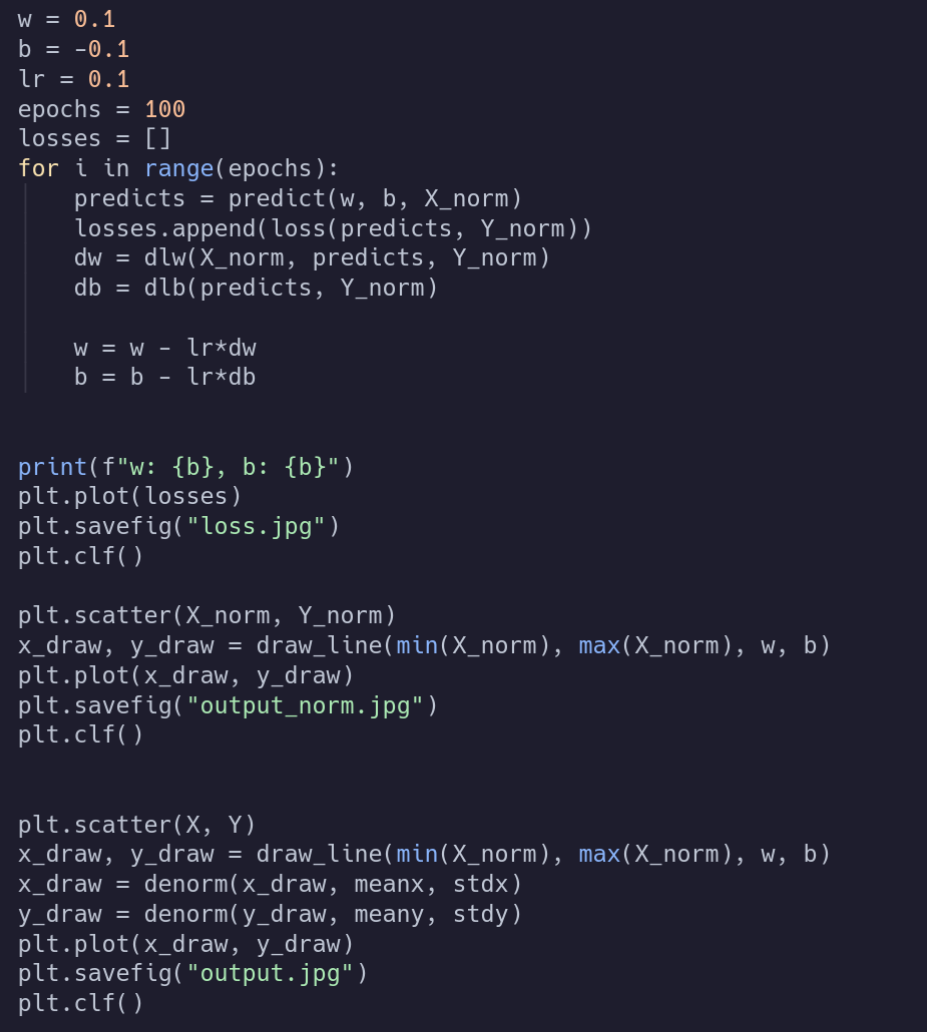
\includegraphics[width=0.6\linewidth]{training_norm.png}
    \caption{Training with normalization}
    \label{fig:enter-label}
\end{figure}

\begin{figure}[H]
    \centering
    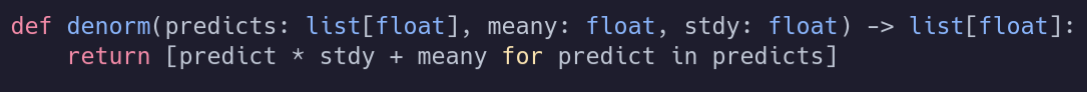
\includegraphics[width=0.75\linewidth]{denorm.png}
    \caption{Denormalization code}
    \label{fig:enter-label}
\end{figure}

We saw that when we train the model on the normalized data, we can use the learning rate of 0.1 (which previously cause divergence) and the loss function converge very quickly. We only need about 20 epochs compare to 4000 epochs of before. We can also see that the model can predict the trend of the normalized and original data very well.

\begin{figure}[H]
\centering
    \begin{subfigure}{0.5\linewidth}
    
        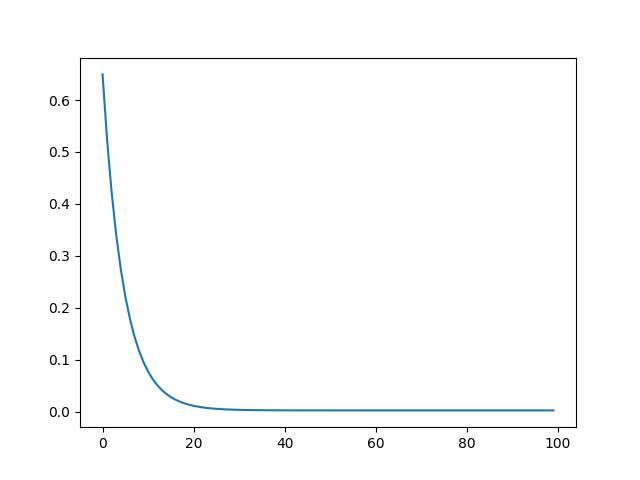
\includegraphics[width=\linewidth]{loss.jpg} 
        \caption{Loss function}
    \end{subfigure}
        
    \begin{subfigure}{0.5\linewidth}
        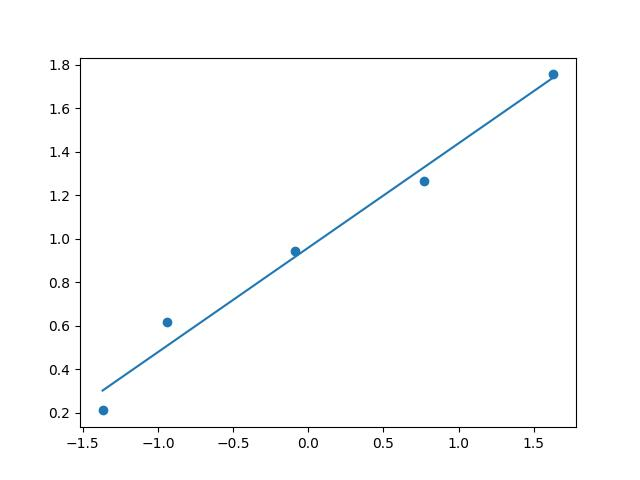
\includegraphics[width=\linewidth]{output_norm.jpg} 
        \caption{Predicted output on the normalized data}
    \end{subfigure}
    
    \begin{subfigure}{0.5\linewidth}
        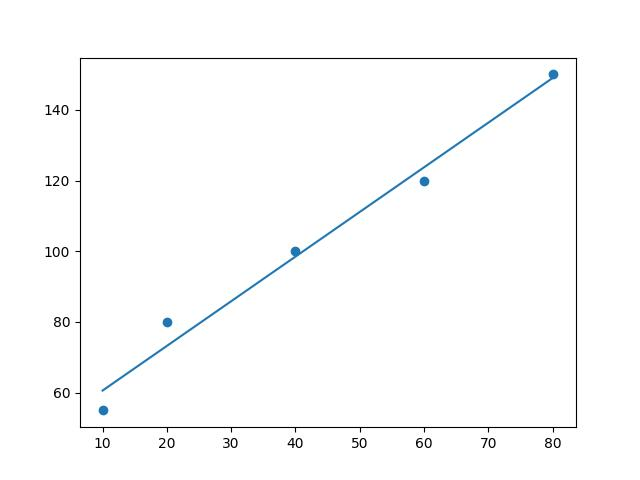
\includegraphics[width=\linewidth]{output.jpg} 
        \caption{Predicted output on the original data}
    \end{subfigure}
    
    \caption{Training results with normalized data}
    \label{fig:enter-label}
\end{figure}

\end{document}
